% PyBaMM Battery Modelling Conference 2026 — 1-page abstract, v8 draft.
% Author: Krishna Chaitanya Vaddepally, Turno (Blubble Pvt. Ltd.)
% Deadline: 2026-07-15 UTC (max 1 A4 page, Arial >= 12 pt).
%
% Theme and presentation preference are NOT printed on the abstract page
% (entered only in the submission form). See memory `v8-scope-frozen-july15`.
%
\documentclass[12pt,a4paper]{article}

\usepackage[T1]{fontenc}
\usepackage{amsmath,amssymb}
\usepackage{helvet}
\renewcommand{\familydefault}{\sfdefault}

\usepackage[a4paper,top=0.7cm,bottom=0.7cm,left=1.3cm,right=1.3cm]{geometry}
\usepackage{graphicx}
\usepackage{caption}
\captionsetup{font=footnotesize,labelfont=bf,labelsep=colon,skip=2pt}
\usepackage{microtype}
\usepackage[hidelinks]{hyperref}
\usepackage{enumitem}
\usepackage{float}
\usepackage{tikz}
\usetikzlibrary{arrows.meta,positioning,shapes.geometric}

\pagestyle{empty}
\setlength{\parindent}{0pt}
\setlength{\parskip}{0.10em}

\begin{document}

\begin{center}
{\bfseries\large Adaptive SoH Forecasting for Second-Life LFP Cells\\
Using PyBaMM-Generated Data and Hybrid Model Selection}\\[0.40em]
\underline{Krishna Chaitanya Vaddepally}\\
\emph{Turno (Blubble Pvt.\ Ltd.), Bengaluru, India}\\
krishna.vaddepally@turno.club
\end{center}

Second-life reuse of retired lithium iron phosphate cells requires rapid
prediction of future degradation for each incoming cell. Rather than
assuming that one forecasting model is optimal for all cells, we combine
exponential extrapolation with a PyBaMM~[1]-trained neural operator and
select between them using early-cycle behaviour.

A short diagnostic and the first $K{=}50$ operating cycles provide the
model context. A Neural ODE~[3] was trained on 490 PyBaMM SPMe
degradation trajectories generated around seven anchor cells from three
LFP suppliers (CALB, EVE, REPT) on Prada2013 chemistry~[2], using
trajectory-grouped train/validation partitions. In parallel, an
exponential model was fitted to the same context; its first-80\%-fit,
last-20\%-prediction context-holdout residual indicates departure from
exponential behaviour. A threshold set on synthetic trajectories alone
routes each cell to either forecast (Figure~\ref{fig:selector}).

\begin{figure}[H]
  \centering
  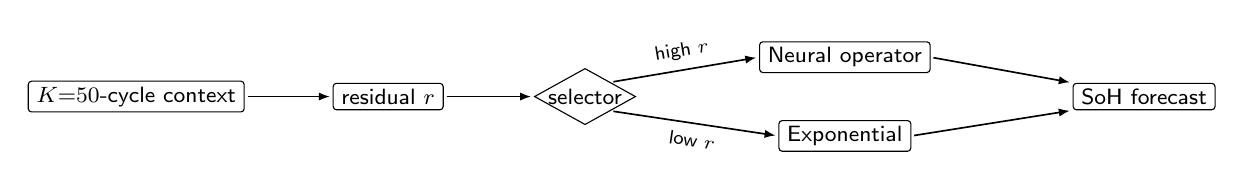
\begin{tikzpicture}[
    every node/.style={font=\footnotesize},
    box/.style={draw,rounded corners=1.2pt,inner xsep=3pt,inner ysep=2pt,
                align=center},
    dec/.style={draw,diamond,aspect=1.8,inner sep=0pt,align=center},
    arr/.style={-{Latex[length=1.4mm]},semithick,shorten <=1pt,shorten >=1pt},
    x=1mm,y=1mm,
  ]
    \node[box] (ctx) at (0,0)   {$K{=}50$-cycle context};
    \node[box] (res) at (32,0)  {residual $r$};
    \node[dec] (dec) at (57,0)  {selector};
    \node[box] (op)  at (90,5)  {Neural operator};
    \node[box] (exp) at (90,-5) {Exponential};
    \node[box] (out) at (128,0) {SoH forecast};
    \draw[arr] (ctx) -- (res);
    \draw[arr] (res) -- (dec);
    \draw[arr] (dec.north east) -- node[above,sloped,font=\scriptsize]{high $r$} (op.west);
    \draw[arr] (dec.south east) -- node[below,sloped,font=\scriptsize]{low $r$} (exp.west);
    \draw[arr] (op.east) -- (out.north west);
    \draw[arr] (exp.east) -- (out.south west);
  \end{tikzpicture}
  \caption{Adaptive selector. A context-holdout residual $r$ (exp fit on
  the first 80\% of the $K{=}50$ context, RMSE on the last 20\%) routes
  each cell to either the PyBaMM-trained neural operator (high $r$) or
  exponential extrapolation (low $r$); the threshold is set on
  synthetic trajectories only.}
  \label{fig:selector}
\end{figure}

Across three external cells excluded from operator training, exponential
and neural forecasts achieved mean SoH RMSEs of 0.70 and 0.80 percentage
points, respectively (Figure~\ref{fig:trajectories}). Across these three
cells, the frozen residual-based selector chose the lower-error model
for all three and reduced mean RMSE to \textbf{0.47 percentage points},
a 33\% improvement relative to the best fixed strategy. Exponential
extrapolation performed best for CALB\_0029 and REPT\_0028, whereas the
neural operator performed best for EVE\_0003.

\begin{figure}[H]
  \centering
  \IfFileExists{figures/heldout_v8_selector_trajectories.pdf}{%
    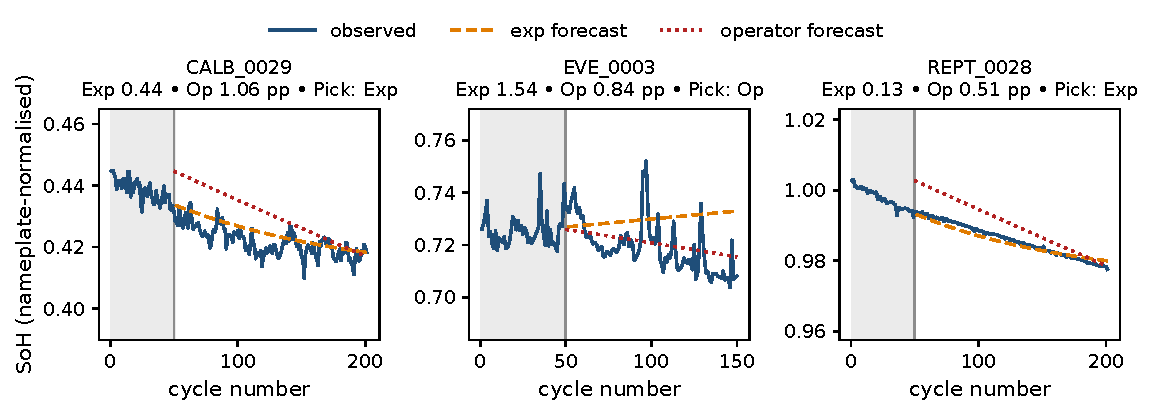
\includegraphics[width=\textwidth]{figures/heldout_v8_selector_trajectories.pdf}%
  }{%
    \fbox{\parbox[c][0.6cm][c]{0.9\textwidth}{\centering\footnotesize
      [placeholder]}}%
  }
  \caption{Forecasts evaluated against measured post-context SoH for
  three external cells. Grey shading denotes the $K{=}50$ context
  window; orange dashed and red dotted lines show exponential and
  neural-operator forecasts, respectively. Panels use independent
  y-axis ranges.}
  \label{fig:trajectories}
\end{figure}

Matched ablations showed little additional benefit from explicit
degradation-parameter conditioning: full-, no- and reduced-$\theta$
operators achieved mean RMSEs of 0.80, 0.82 and 0.90 percentage points,
respectively. These results suggest that matching model complexity to
observed early-cycle behaviour may be more effective than applying one
forecasting model uniformly across heterogeneous second-life cells.
Evaluation is currently limited to three external cells, and
longer-horizon projections require additional experimental validation.

\vspace{-0.4em}
{\scriptsize
[1]~V.~Sulzer et al., \emph{J.\ Open Res.\ Software} \textbf{9} (2021), 14.
\textbullet\ [2]~M.~Prada et al., \emph{J.\ Power Sources} \textbf{219} (2012),
353--362. \textbullet\ [3]~R.\,T.\,Q.~Chen et al., \emph{NeurIPS} (2018).
}

\end{document}
